\documentclass[a4paper,12pt]{article} 


\usepackage[T2A]{fontenc}			
\usepackage[utf8]{inputenc}			
\usepackage[english,russian]{babel}	

\usepackage{graphicx, scalerel}    
\usepackage{wrapfig}               
\usepackage[14pt]{extsizes}        
\usepackage[warn]{mathtext}       
\usepackage{indentfirst}      
\usepackage[margin = 25mm]{geometry}
\usepackage[table,xcdraw]{xcolor} 
\usepackage{amsmath,amsfonts,amssymb,amsthm,mathtools}
\usepackage{wasysym}                
\usepackage{upgreek}                
\usepackage{caption}
\usepackage{multirow}
\captionsetup{labelsep=period}
\usepackage[font=small,labelfont=bf]{caption}
\usepackage{gensymb}
\usepackage{icomma}

\usepackage[unicode, pdftex]{hyperref}
\usepackage{tikz}
\usetikzlibrary{positioning}
\usepackage{fancyhdr}
\pagestyle{fancy}
\setlength\fboxsep{3pt} % Отступ рамки \fbox{} от рисунка
\setlength\fboxrule{1pt} % Толщина линий рамки \fbox{}
\usepackage{tocloft}

\begin{document}
	\newcommand{\HRule}{\rule{\linewidth}{0.7mm}} % Defines a new command for the horizontal lines, change thickness here

\begin{center}
	\large\textbf{Московский Физико-Технический Институт}\\
	\large\textbf{(государственный университет)}
	
	\vfill
	
	
	
	\Large Лабораторная работа 5.1.2
	%----------------------------------------------------------------------------------------
	%	TITLE SECTION
	%----------------------------------------------------------------------------------------
	
	\HRule
	\\[0.4cm]
	{ \huge \bfseries Исследование эффекта Комптона}
	\\[0.4cm] % Title of your document
	\HRule
	\\[0.5cm]
	
	\ \\
	\textbf{\large Автор:} \\	
	\large Овсянников Михаил Б01-008\\
	\vfill
	\hspace*{-0.8 cm}
\includegraphics[width=100 pt]{./Include/frkt_logo.pdf}\\
	\large Долгопрудный, 2022
\end{center}

\thispagestyle{empty}

\newpage
\setcounter{page}{2}
\fancyfoot[c]{\thepage}
\fancyhead[L] {Лабораторная работа 5.1.2}
\fancyhead[R] {Исследование эффекта Комптона}

	\newpage
	
	\tableofcontents
	
	
	
	\newpage
	\textbf{Цель работы:} исследовать спектральные закономерности в оптическом спектре водорода. По результатам измерений вычислить постоянную Ридберга для водорода.
	
	\tocsection{Теоретические сведения}
	Атом водорода является простейшей атомной системой; для него уравнение Шредингера может быть решено точно. Поэтому спектр атома водорода является предметом тщательного экспериментального и теоретического исследования.
	
	Объяснение структуры спектра излучения атомов требует знания схемы атомных энергетических уровней, что, в свою очередь, требует решения задачи о движении электрона в эффективном поле атома. Для атома водорода и водородоподобных (одноэлектронных) атомов определение энергетических уровней значительно упрощается, так как квантово-механическая задача об относительном движении электрона (заряд $-e$, масса $m_e$) и ядра (заряд $Ze$, масса $M$) сводится к задаче о движении частицы с эффективной массой $\mu = m_e M/(m_e + M)$ в кулоновском поле $-Ze^2/r$. Однако даже для водородоподобных атомов это решение не является простым.

	
	Длины волн спектральных линий водородоподобного атома описываются формулой
	\begin{equation}
		\frac{1}{\lambda_{mn}} = RZ^2\left(\frac{1}{n^2} - \frac{1}{m^2}\right),
	\end{equation}
	
	\noindent где $R$ -- константа, называемая постоянной Ридберга, а $m$ и $n$ -- целые числа. Эта формула достаточно правильно описывает экспериментальные значения линий водорода при $R = 109 677,6$ см$^{-1}$.
	
	В данной работе изучается серия Бальмера, линии которой лежат в видимой области. Для серии Бальмера $n = 2$. Величина $m$ для первых четырех линий этой серии принимает значение $3, 4, 5, 6$. Эти линии обозначаются символами $H_\alpha$, $H_\beta$, $H_\gamma$, $H_\delta$.
	
	Энергия уровня с квантовым числом $n$ определяется формулой:
	\begin{equation}
		E_n = -\frac{m_e Z^2 e^4}{2\hbar^2}\frac{1}{n^2} = -R\frac{Z^2}{n^2}.
	\end{equation}

	\newpage
	\tocsection{Экспериментальная установка}
	Для измерения длин волн спектральных линий в работе используется стеклянно-призменный монохроматор-спектрометр УМ-2, предназначенный для спектральных исследований в диапазоне от 0,38 до 1,00 мкм.
	\begin{figure}[h!]
		\centering
		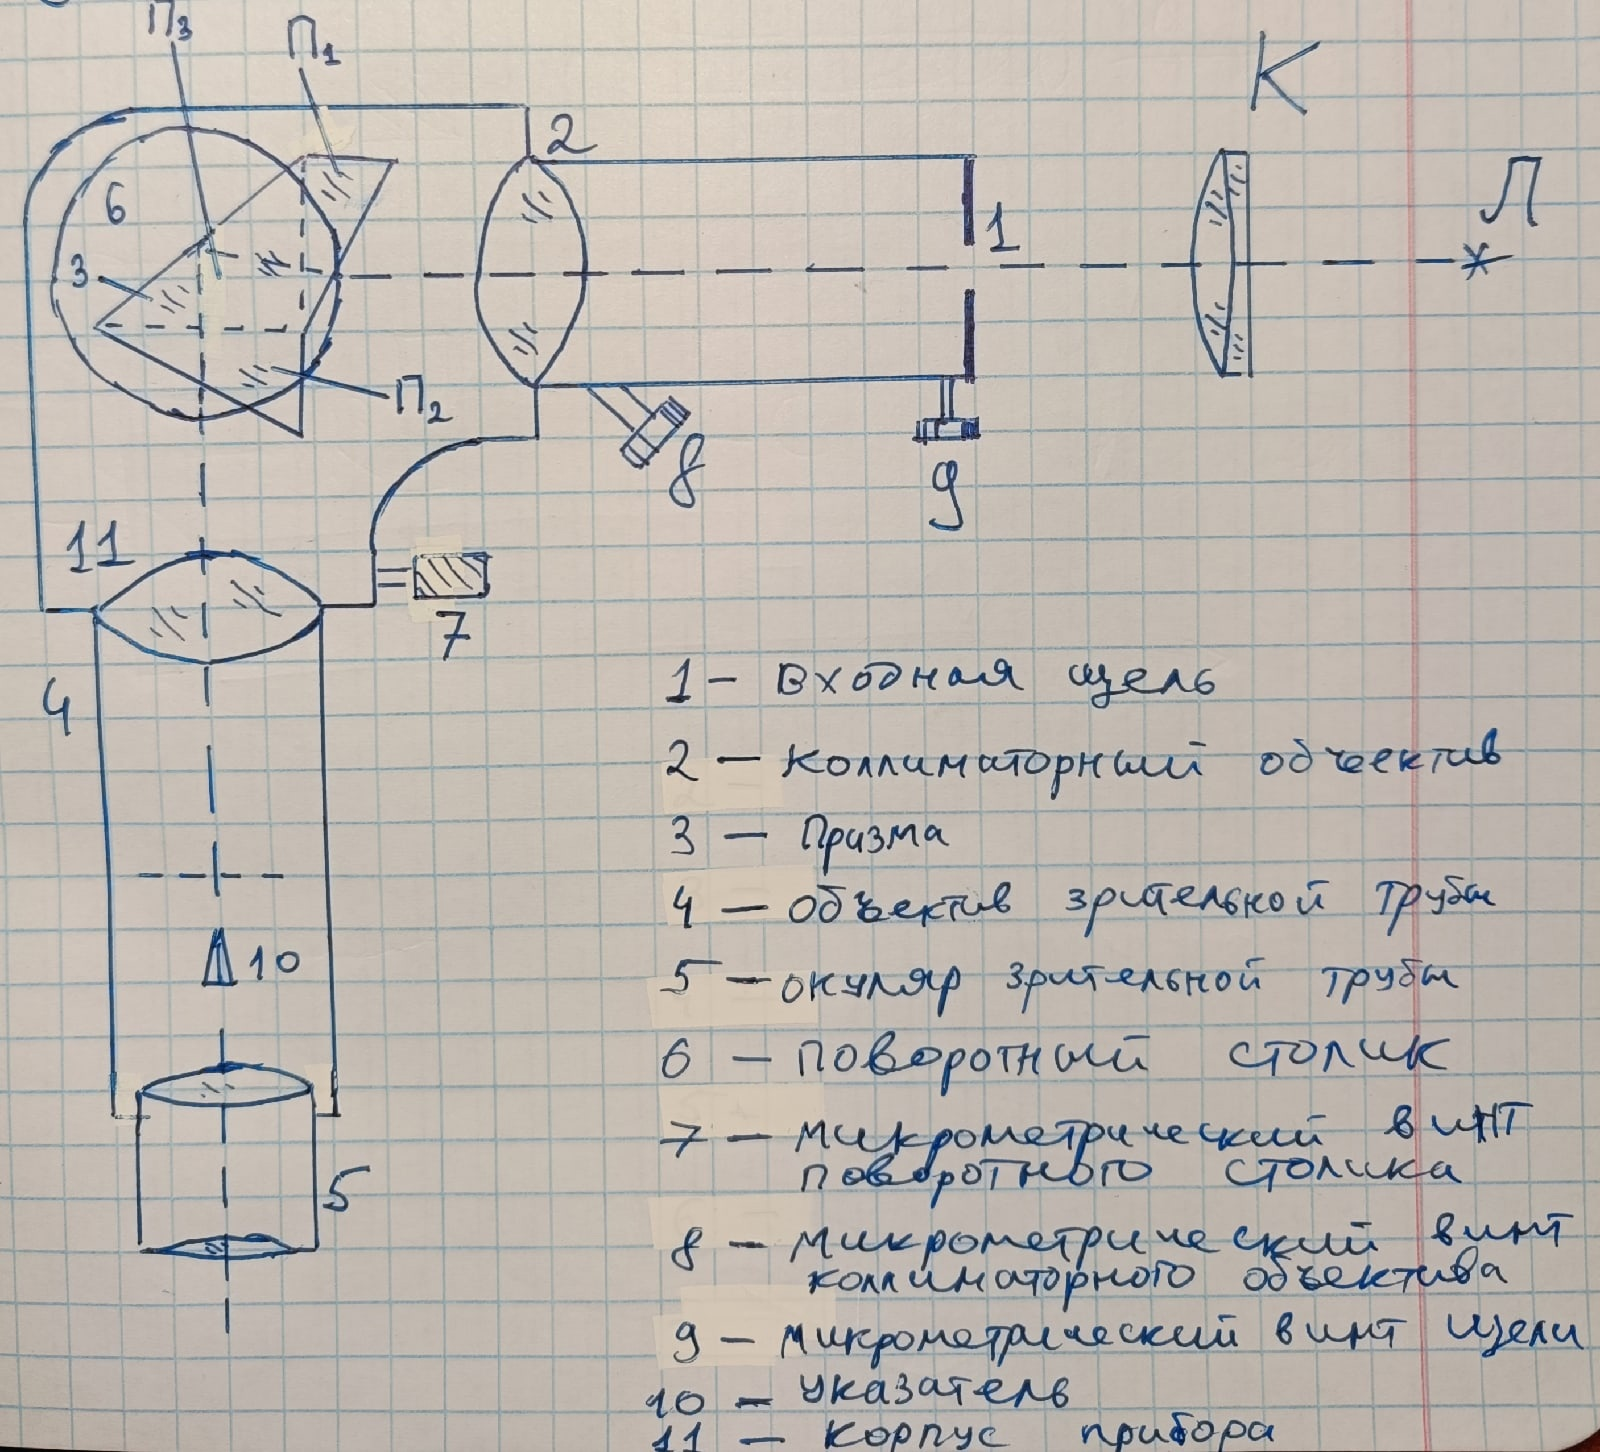
\includegraphics[width=\linewidth]{Pictures/State}
		\caption{Устройство монохроматора УМ-2}
	\end{figure}
	Первые две призмы с преломляющими углами $30^\circ$ изготовлены из тяжелого флинта, обладающего большой дисперсией. Промежуточная призма П$_3$ сделана из крона. Лучи отражаются от ее гипотенузной грани и поворачиваются на $90^\circ$. Благодаря такому устройству дисперсии призм П$_1$ и П$_2$ складываются.
	
	Для отсчета положения спектральной линии ее центр совмещается с острием указателя. Отсчет проводится по делениям барабана.
	
	Для градуировки в коротковолновой части спектра удобно применять ртутную лампу ПРК-4, а в длинноволновой и средней части спектра -- неоновую лампу. 
	
	Для увеличения яркости интересующих нас линий атомарного водорода в состав газа, которым заполняют трубку при ее изготовлении, добавляют пары воды. Молекулы воды в электрическом разряде разлагаются, образуя атомарный водород. Трубка заполняется газом до давления 5–10 Тор.
	
	\tocsection{Ход работы}
	\begin{enumerate}
		\item Проградуируем спектрометр УМ-2 по спектрам неона и ртути. Отсчитываем угол по барабану. Погрешность измерения углов $\sigma_{\theta} = 5^\circ$. Результаты для неона и ртути запишем в таблицу \ref{HydrogenSpectre_GradsTable}.

	
		\begin{table}[h!]
			\centering
			\resizebox{\columnwidth}{!}{%
				\begin{tabular}{|rrr|rrrrrr}
					\cline{1-3} \cline{7-9}
					\multicolumn{3}{|c|}{Неон}                                                                                                &                      &                      & \multicolumn{1}{r|}{} & \multicolumn{3}{c|}{Ртуть}                                                                                               \\ \cline{1-3} \cline{7-9} \multicolumn{1}{|c|}{} & \multicolumn{1}{c|}{} & \multicolumn{1}{c|}{} & \multicolumn{1}{c}{} & \multicolumn{1}{c}{} & \multicolumn{1}{c|}{} & \multicolumn{1}{c|}{} & \multicolumn{1}{c|}{} & \multicolumn{1}{c|}{} \\ 
					\multicolumn{1}{|c|}{Линия} & \multicolumn{1}{c|}{Угол $\theta ^\circ$} & \multicolumn{1}{c|}{Длина волны, \AA} & \multicolumn{1}{c}{} & \multicolumn{1}{c}{} & \multicolumn{1}{c|}{} & \multicolumn{1}{c|}{Линия} & \multicolumn{1}{c|}{Угол $\theta ^\circ$} & \multicolumn{1}{c|}{Длина волны, \AA} \\ \cline{1-3} \cline{7-9} 
					\multicolumn{1}{|r|}{1}     & \multicolumn{1}{r|}{2542}            & 7032                                                 &                      &                      & \multicolumn{1}{r|}{} & \multicolumn{1}{r|}{K1}    & \multicolumn{1}{r|}{2506}            & \multicolumn{1}{r|}{6907}                            \\ \cline{1-3} \cline{7-9} 
					\multicolumn{1}{|r|}{2}     & \multicolumn{1}{r|}{2518}            & 6929                                                 &                      &                      & \multicolumn{1}{r|}{} & \multicolumn{1}{r|}{K2}    & \multicolumn{1}{r|}{2270}            & \multicolumn{1}{r|}{6234}                            \\ \cline{1-3} \cline{7-9} 
					\multicolumn{1}{|r|}{3}     & \multicolumn{1}{r|}{2444}            & 6717                                                 &                      &                      & \multicolumn{1}{r|}{} & \multicolumn{1}{r|}{1}     & \multicolumn{1}{r|}{2068}            & \multicolumn{1}{r|}{5791}                            \\ \cline{1-3} \cline{7-9} 
					\multicolumn{1}{|r|}{4}     & \multicolumn{1}{r|}{2436}            & 6678                                                 &                      &                      & \multicolumn{1}{r|}{} & \multicolumn{1}{r|}{2}     & \multicolumn{1}{r|}{2056}            & \multicolumn{1}{r|}{5770}                            \\ \cline{1-3} \cline{7-9} 
					\multicolumn{1}{|r|}{5}     & \multicolumn{1}{r|}{2410}            & 6599                                                 &                      &                      & \multicolumn{1}{r|}{} & \multicolumn{1}{r|}{3}     & \multicolumn{1}{r|}{1876}            & \multicolumn{1}{r|}{5461}                            \\ \cline{1-3} \cline{7-9} 
					\multicolumn{1}{|r|}{6}     & \multicolumn{1}{r|}{2386}            & 6533                                                 &                      &                      & \multicolumn{1}{r|}{} & \multicolumn{1}{r|}{4}     & \multicolumn{1}{r|}{1452}            & \multicolumn{1}{r|}{4916}                            \\ \cline{1-3} \cline{7-9} 
					\multicolumn{1}{|r|}{7}     & \multicolumn{1}{r|}{2376}            & 6507                                                 &                      &                      & \multicolumn{1}{r|}{} & \multicolumn{1}{r|}{5}     & \multicolumn{1}{r|}{786}             & \multicolumn{1}{r|}{4358}                            \\ \cline{1-3} \cline{7-9} 
					\multicolumn{1}{|r|}{8}     & \multicolumn{1}{r|}{2338}            & 6402                                                 &                      &                      & \multicolumn{1}{r|}{} & \multicolumn{1}{r|}{6}     & \multicolumn{1}{r|}{226}             & \multicolumn{1}{r|}{4047}                            \\ \cline{1-3} \cline{7-9} 
					\multicolumn{1}{|r|}{9}     & \multicolumn{1}{r|}{2330}            & 6383                                                 &                      &                      &                       &                            &                                      &                                                      \\ \cline{1-3}
					\multicolumn{1}{|r|}{10}    & \multicolumn{1}{r|}{2310}            & 6334                                                 &                      &                      &                       &                            &                                      &                                                      \\ \cline{1-3}
					\multicolumn{1}{|r|}{11}    & \multicolumn{1}{r|}{2296}            & 6305                                                 &                      &                      &                       &                            &                                      &                                                      \\ \cline{1-3}
					\multicolumn{1}{|r|}{12}    & \multicolumn{1}{r|}{2284}            & 6267                                                 &                      &                      &                       &                            &                                      &                                                      \\ \cline{1-3}
					\multicolumn{1}{|r|}{13}    & \multicolumn{1}{r|}{2264}            & 6217                                                 &                      &                      &                       &                            &                                      &                                                      \\ \cline{1-3}
					\multicolumn{1}{|r|}{14}    & \multicolumn{1}{r|}{2244}            & 6164                                                 &                      &                      &                       &                            &                                      &                                                      \\ \cline{1-3}
					\multicolumn{1}{|r|}{15}    & \multicolumn{1}{r|}{2234}            & 6143                                                 &                      &                      &                       &                            &                                      &                                                      \\ \cline{1-3}
					\multicolumn{1}{|r|}{16}    & \multicolumn{1}{r|}{2214}            & 6096                                                 &                      &                      &                       &                            &                                      &                                                      \\ \cline{1-3}
					\multicolumn{1}{|r|}{17}    & \multicolumn{1}{r|}{2204}            & 6074                                                 &                      &                      &                       &                            &                                      &                                                      \\ \cline{1-3}
					\multicolumn{1}{|r|}{18}    & \multicolumn{1}{r|}{2186}            & 6030                                                 &                      &                      &                       &                            &                                      &                                                      \\ \cline{1-3}
					\multicolumn{1}{|r|}{19}    & \multicolumn{1}{r|}{2156}            & 5976                                                 &                      &                      &                       &                            &                                      &                                                      \\ \cline{1-3}
					\multicolumn{1}{|r|}{20}    & \multicolumn{1}{r|}{2146}            & 5945                                                 &                      &                      &                       &                            &                                      &                                                      \\ \cline{1-3}
					\multicolumn{1}{|r|}{21}    & \multicolumn{1}{r|}{2114}            & 5882                                                 &                      &                      &                       &                            &                                      &                                                      \\ \cline{1-3}
					\multicolumn{1}{|r|}{22}    & \multicolumn{1}{r|}{2098}            & 5852                                                 &                      &                      &                       &                            &                                      &                                                      \\ \cline{1-3}
					\multicolumn{1}{|r|}{23}    & \multicolumn{1}{r|}{1836}            & 5401                                                 &                      &                      &                       &                            &                                      &                                                      \\ \cline{1-3}
					\multicolumn{1}{|r|}{24}    & \multicolumn{1}{r|}{1800}            & 5341                                                 &                      &                      &                       &                            &                                      &                                                      \\ \cline{1-3}
					\multicolumn{1}{|r|}{25}    & \multicolumn{1}{r|}{1796}            & 5331                                                 &                      &                      &                       &                            &                                      &                                                      \\ \cline{1-3}
				\end{tabular}%
			}
		\caption{Градуировка по спектрам неона и ртути}
		\label{HydrogenSpectre_GradsTable}
		\end{table}

		Построим градуировочный график, основываясь на этих данных.

		
		\begin{figure}[h!]
			\centering
			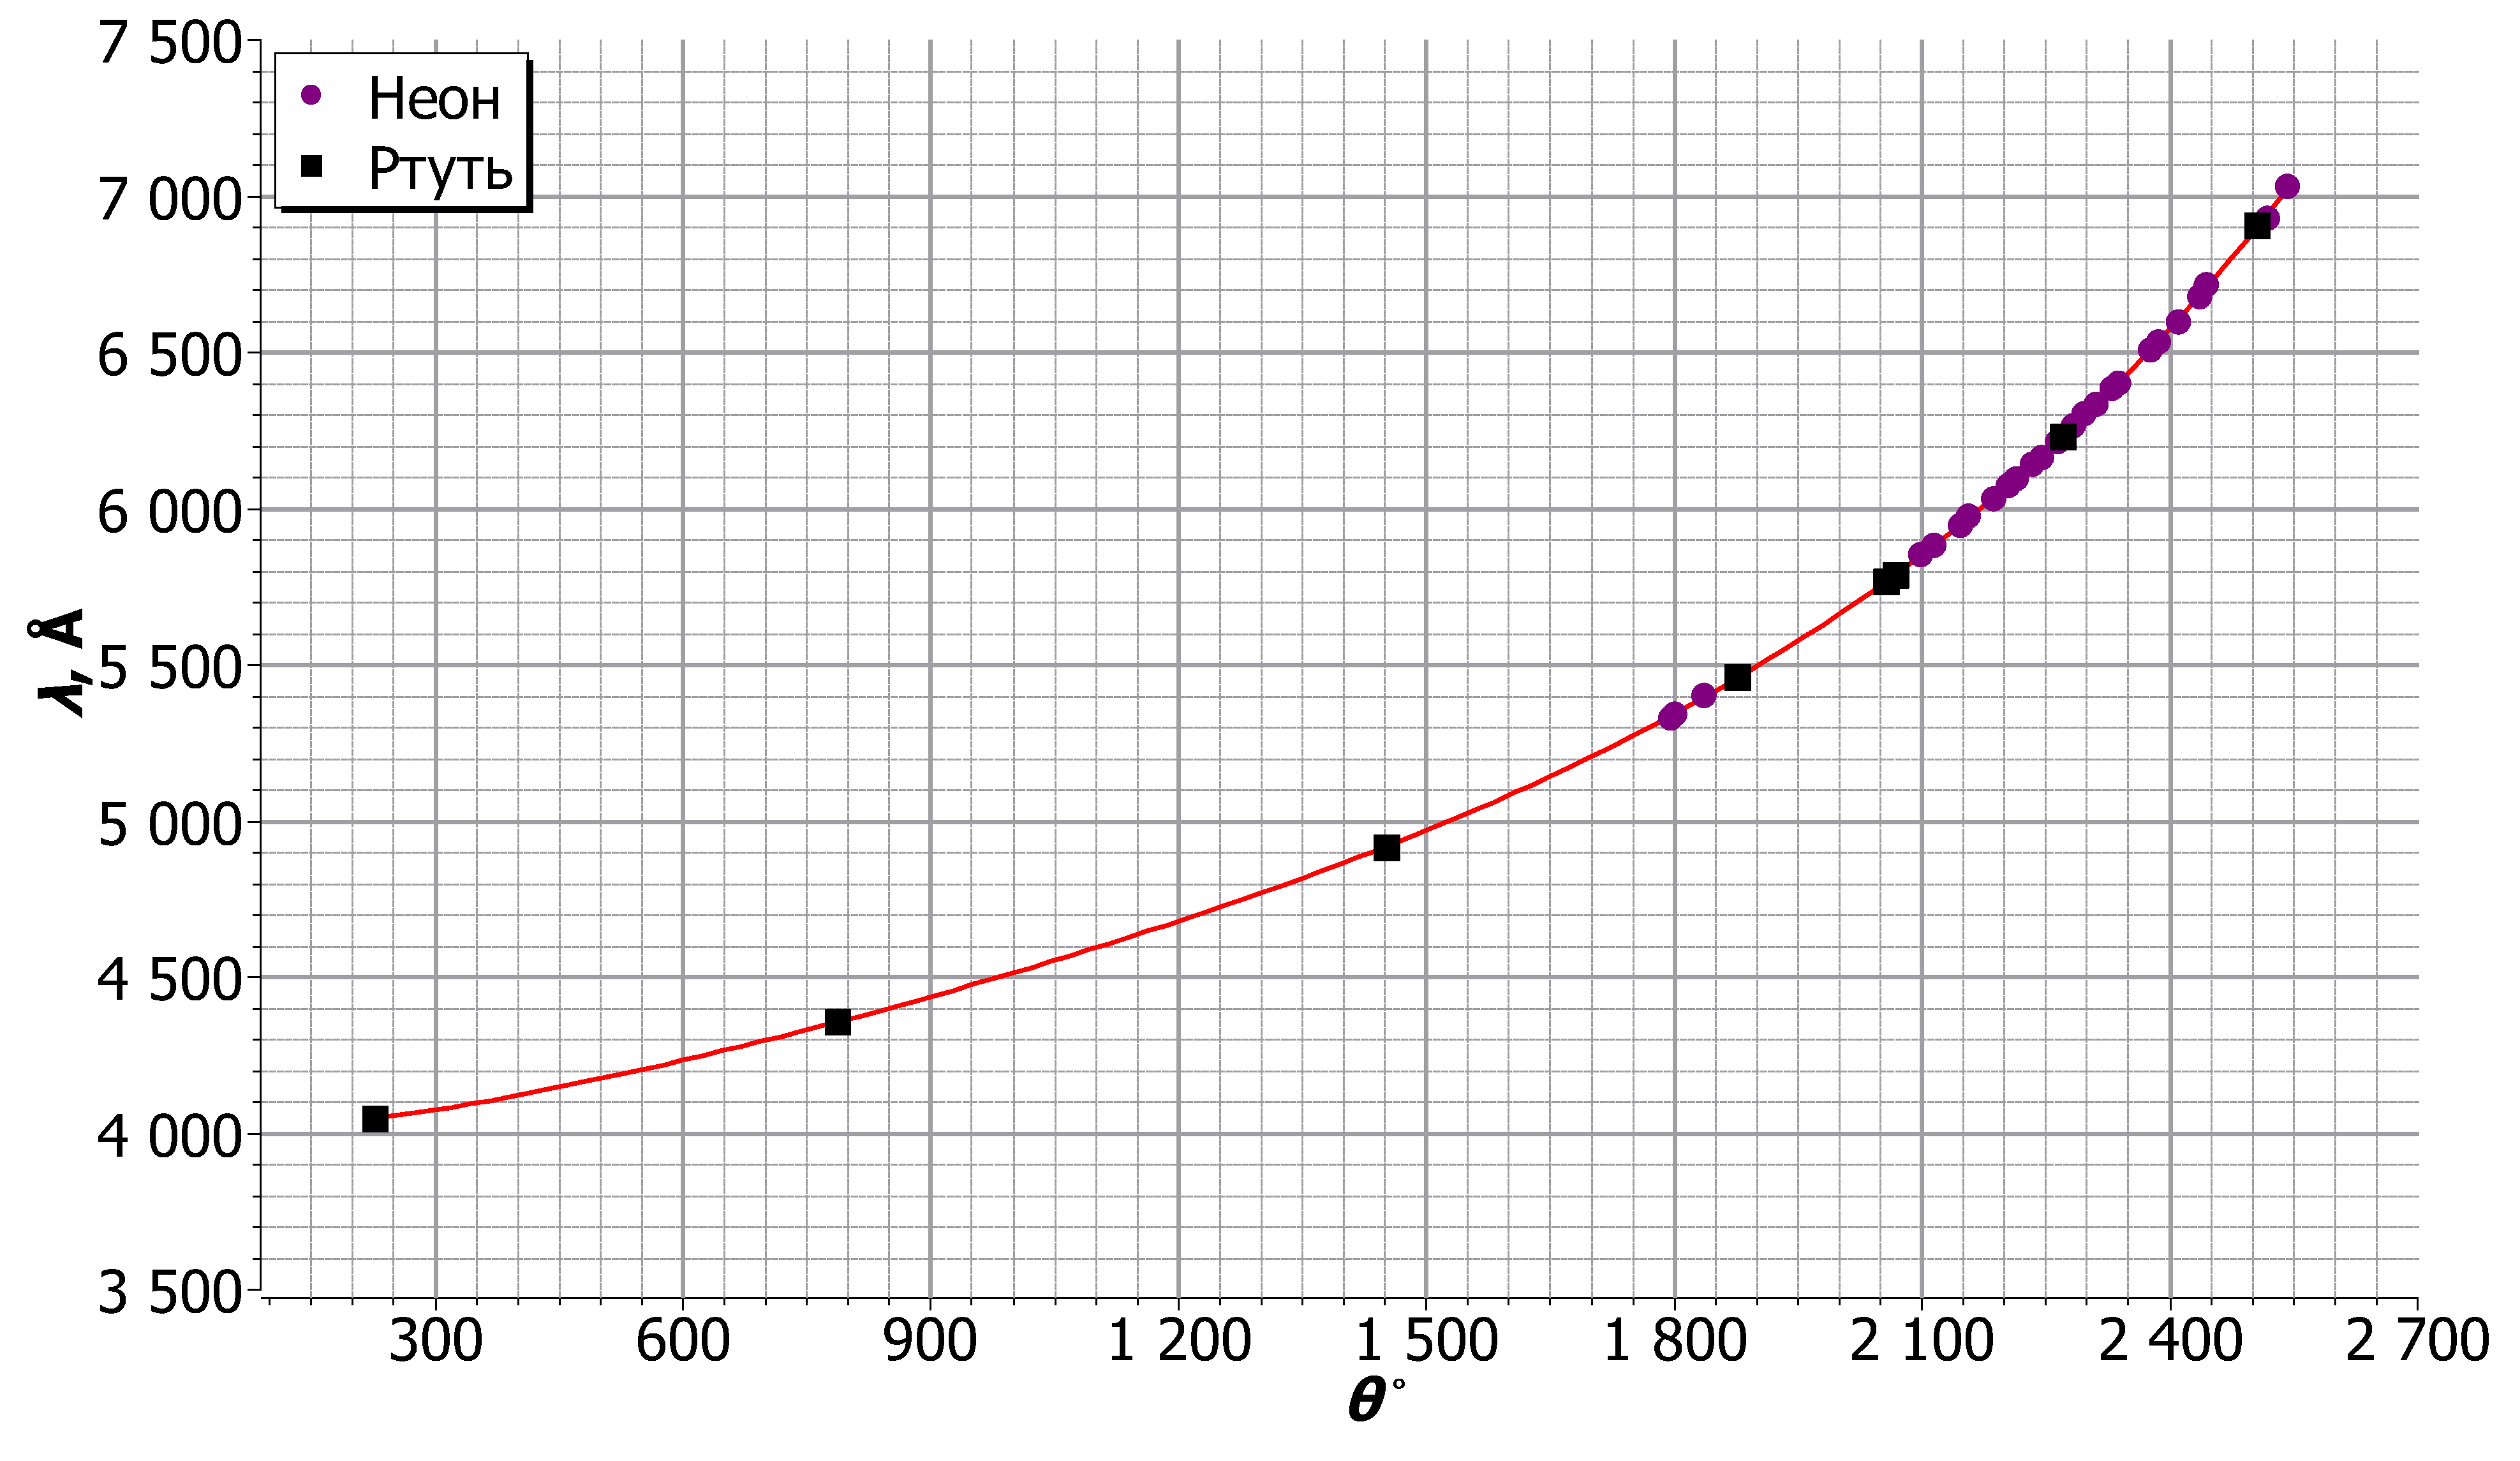
\includegraphics[width=\linewidth]{Pictures/Lambda(theta).pdf}
			\caption{Зависимость $\lambda(\theta)$}
		\end{figure}
	
		Использовалась аппроксимация:
		\begin{equation*}
			\lambda(\theta) = A + \frac{B}{\theta - C}.
		\end{equation*}
		Из расчетов получаем следующее:
		\begin{itemize}
			\item $A = (2343 \pm 4)$ \AA
			
			\item $B = (-6200 \pm 14) \cdot 10^3$ \AA
			
			\item $C = (3865 \pm 2)$
			
		\end{itemize}

		
 		\item Измерим положения линий атома водорода. Результаты пишем в таблицу \ref{HydrogenSpectre_LinesTable}.
	
		\begin{table}[h!]
			\centering
				\begin{tabular}{|r|r|}
					\hline
					Линия      & Угол $\theta ^\circ$ \\ \hline
					$H_\alpha$ & 2394                 \\ \hline
					$H_\beta$  & 1404                 \\ \hline
					$H_\gamma$ & 756                  \\ \hline
					$H_\delta$ & 338                  \\ \hline
				\end{tabular}
			\caption{Линии атома водорода}
			\label{HydrogenSpectre_LinesTable}
		\end{table}

	Используя аппроксимирующую формулу и градуировочный график, найдем значения длин волн для этих линий. Погрешность для каждой:
	\begin{equation*}
		\sigma_\lambda = \sqrt{\left(\frac{\partial \lambda}{\partial A}\right)^2 \sigma_A ^2 + \left(\frac{\partial \lambda}{\partial B}\right)^2 \sigma_B ^2 + \left(\frac{\partial \lambda}{\partial C}\right)^2 \sigma_C ^2 + \left(\frac{\partial \lambda}{\partial \theta}\right)^2 \sigma_\theta ^2}
	\end{equation*}
	\begin{equation*}
		\sigma_{\lambda} = \sqrt{\sigma_A^2 + \frac{\sigma_B^2}{(\theta - C)^2} + \frac{B^2 \sigma_C^2}{(\theta - C)^4} + \frac{B^2 \sigma_\theta^2}{(\theta - C)^4}}
	\end{equation*}


	\begin{table}[h!]
		\centering
			\begin{tabular}{|r|r|r|r|}
				\hline
				&  &  & \multicolumn{1}{r|}{} \\ 
				Линия      & Угол $\theta ^\circ$ & Длина волны $\lambda$, \AA & \multicolumn{1}{r|}{Табличное значение $\lambda_\text{табл}$, \AA} \\ \hline
				$H_\alpha$ & 2394                 & $6560 \pm 20$                             & 6563                                                                                        \\ \hline
				$H_\beta$  & 1404                 & $4862 \pm 9$                              & 4861                                                                                        \\ \hline
				$H_\gamma$ & 756                  & $4338 \pm 7$                              & 4340                                                                                        \\ \hline
				$H_\delta$ & 338                  & $4101 \pm 6$                              & 4102                                                                                        \\ \hline
			\end{tabular}
	\caption{Сводная таблица по линиям атома водорода}
	\end{table}

	Как видим, результаты чрезвычайно близки к табличным. Ошибка определения длин волн составляет $\thicksim 0,1-0,3\%$.

	\item Теперь рассчитаем постоянную Ридберга $R$ для каждой линии. Результаты в таблице \ref{HydrogenSpectre_RydbergTable}.
	
	
	\begin{table}[h!]
		\centering
			\begin{tabular}{|r|r|r|r|}
				\hline
				&  &  & \multicolumn{1}{r|}{} \\ 
				Линия      & Угол $\theta ^\circ$ & Длина волны $\lambda$, \AA & \multicolumn{1}{r|}{Постоянная Ридберга $R$, см$^{-1}$} \\ \hline
				$H_\alpha$ & 2394                 & $6560 \pm 20$                             & $109756 \pm 300$ \iffalse 335 \fi                                         \\ \hline
				$H_\beta$  & 1404                 & $4862 \pm 9$                              & $109679 \pm 200$ \iffalse 203 \fi                                         \\ \hline
				$H_\gamma$ & 756                  & $4338 \pm 7$                              & $109772 \pm 200$ \iffalse 177 \fi                                         \\ \hline
				$H_\delta$ & 338                  & $4101 \pm 6$                              & $109726 \pm 200$ \iffalse 187 \fi                                         \\ \hline
			\end{tabular}
		\caption{Значение постоянной Ридберга, рассчитанное по линиям водорода}
		\label{HydrogenSpectre_RydbergTable}
	\end{table}
	
	В среднем получаем:
	\begin{equation*}
		\boxed{R = (109733 \pm 100) \text{ см}^{-1}}  \iffalse 117 \fi
	\end{equation*}

	Попробуем задействовать сразу все линии, чтобы разово вычислить постоянную Ридберга.
	Построим график такой вот зависимости величин $\frac{1}{\lambda} = f\left(\frac{1}{n^2} - \frac{1}{m^2}\right)$ и по наклону найдем значение $R$. Поскольку $n$ и $m$ -- это целые числа, то погрешности по оси абсцисс нет. Вдобавок, мы знаем погрешность для каждого значения $1/\lambda$. Именно поэтому выбираем метод построения $\chi^2$.

	
	
	\begin{table}[h!]
		\centering
			\begin{tabular}{|r|r|r|r|r|}
				\hline
				& & & & \\
				Линия      & Длина волны $\lambda$, \AA & $\sigma_\lambda$, \AA & $1/\lambda$, $10^{-4}$ \AA$^{-1}$ & $\sigma_{1/\lambda}$, $10^{-4}$ \AA$^{-1}$ \\ \hline
				$H_\alpha$ & 6560                                      & 20                                   & 1,524                                             & 0,005                                                     \\ \hline
				$H_\beta$  & 4862                                      & 9                                    & 2,057                                             & 0,004                                                     \\ \hline
				$H_\gamma$ & 4338                                      & 7                                    & 2,305                                             & 0,004                                                     \\ \hline
				$H_\delta$ & 4101                                      & 6                                    & 2,438                                             & 0,004                                                     \\ \hline
			\end{tabular}
		\caption{Таблица-приготовление для построения графика}
	\end{table}


	В нашем приближении: $1/\lambda = R \cdot \left(\frac{1}{n^2} - \frac{1}{m^2}\right)$.
	\begin{equation*}
		\chi^2 = \sum\limits_{i = 1}^4 \frac{(y_i - kx_i)^2}{\sigma_{y_i}^2} \rightarrow \min \Longrightarrow k = \dfrac{\sum\limits_{i = 1}^4 \dfrac{x_i y_i}{\sigma_{y_i}^2}}{\sum\limits_{i = 1}^4 \dfrac{x_i^2}{\sigma_{y_i}^2}}
	\end{equation*}

	\begin{figure}[h!]
		\centering
		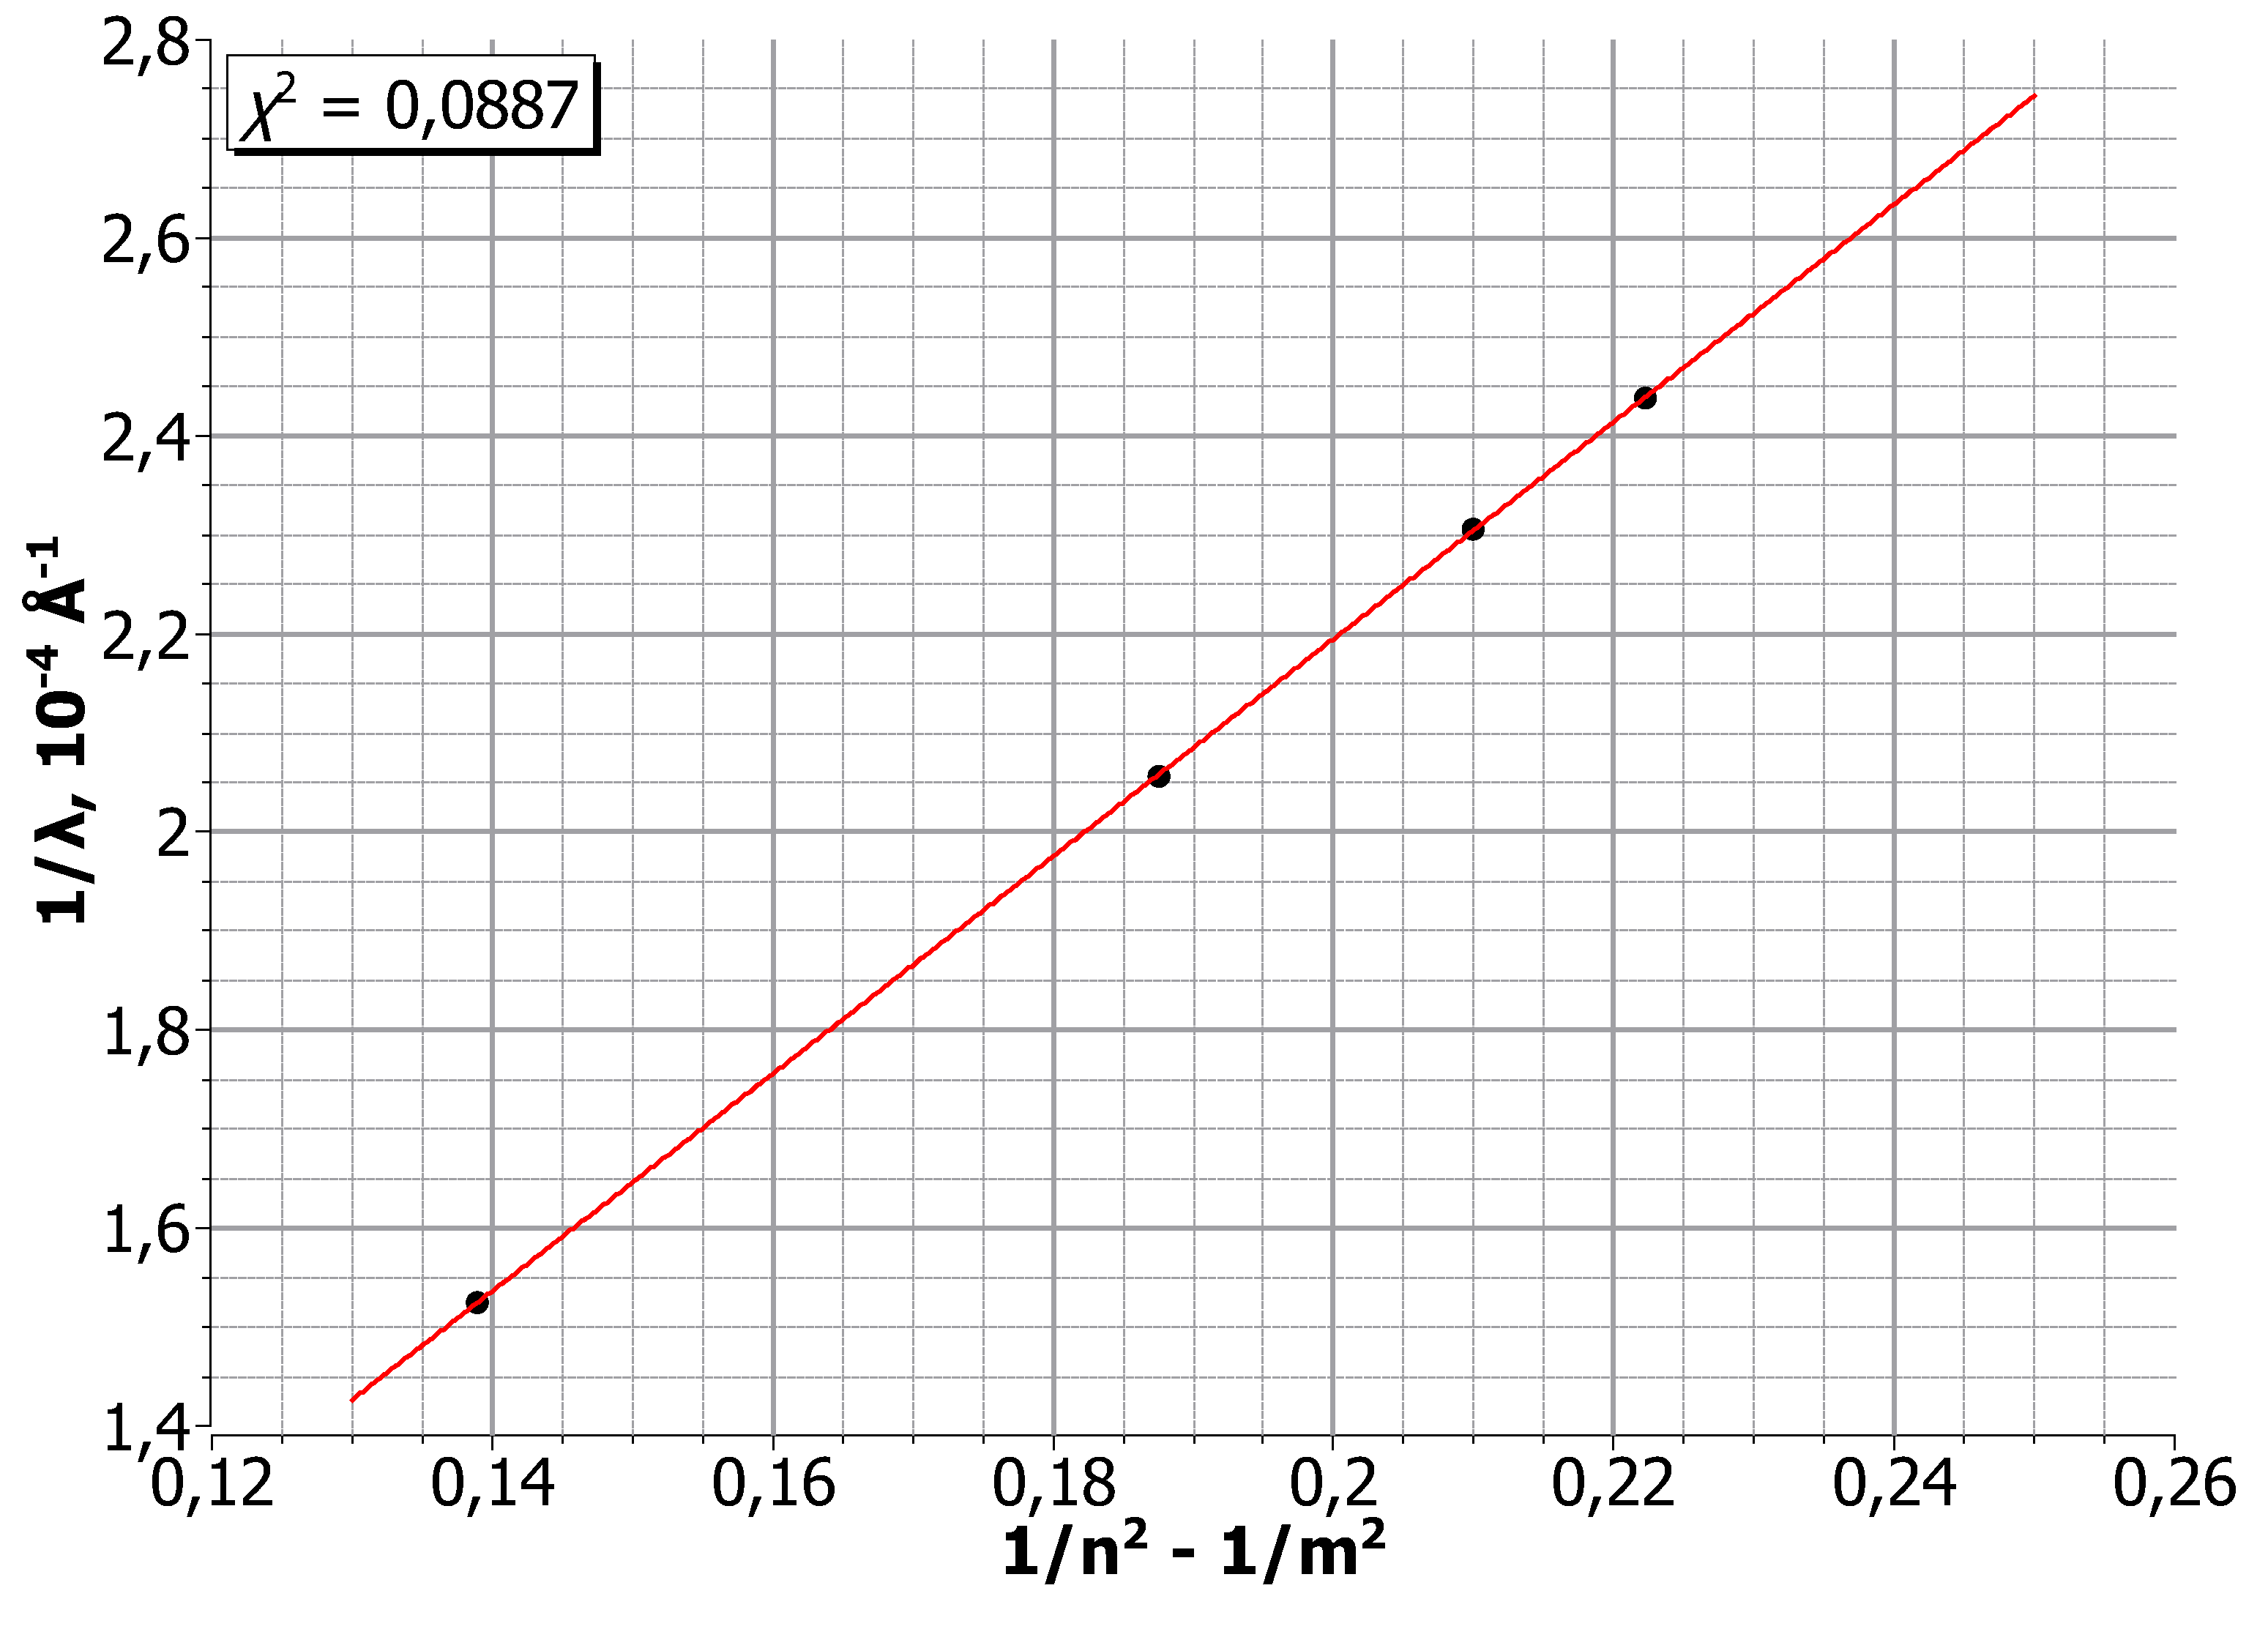
\includegraphics[width=\linewidth]{Pictures/1_over_lambda(Diff).pdf}
		\caption{Зависимость $1/\lambda$ от $1/n^2 - 1/m^2$}
	\end{figure}

	Из графика получаем ($k = R$):
	\begin{equation*}
		\boxed{R = (109736 \pm 100) \text{ см}^{-1}}
	\end{equation*}

	То есть найденное только что значение находится в согласии с ранее посчитанными.
	Учитывая, что табличное значение $R = 109677,6$ см$^{-1}$, то можно сказать, что найденные результаты с отличной точностью совпадают как между друг с другом, так и с табличным значением. 

	\end{enumerate}

	\newpage
	\tocsection{Вывод}
	\begin{table}[h!]
		\centering
		\resizebox{\columnwidth}{!}{%
			\begin{tabular}{rr|r|r|}
				\hline
				\multicolumn{1}{|r|}{}   &   & & \multicolumn{1}{r|}{} \\
				\multicolumn{1}{|r|}{Линия}      & Длина волны $\lambda$, \AA & Табличное значение, \AA & \multicolumn{1}{r|}{Постоянная Ридберга $R$, см$^{-1}$} \\ \hline
				\multicolumn{1}{|r|}{$H_\alpha$} & $6560 \pm 20$  & 6563                            & $109756 \pm 300$                                         \\ \hline
				\multicolumn{1}{|r|}{$H_\beta$}  & $4862 \pm 9$     & 4861                         & $109679 \pm 200$                                         \\ \hline
				\multicolumn{1}{|r|}{$H_\gamma$} & $4338 \pm 7$        & 4340                      & $109772 \pm 200$                                         \\ \hline
				\multicolumn{1}{|r|}{$H_\delta$} & $4101 \pm 6$       & 4102                       & $109726 \pm 200$                                         \\ \hline \cline{3-4}
				& & \textbf{Среднее}                          & $109733 \pm 100$                                        \\ \cline{3-4} 
				& & \textbf{По графику}                       & $109736 \pm 100$                                        \\ \cline{3-4} 
				\multicolumn{1}{l}{}            & & \textbf{Итоговое}                         & $109735 \pm 100$                                        \\ \cline{3-4}
				\multicolumn{1}{l}{}            & & \textbf{Табличное}                         & $109678$                                        \\ \cline{3-4} 
			\end{tabular}
		}
		\caption{Итоговая таблица}
	\end{table}
	
	
	В данной работе мы исследовали спектральные закономерности в оптическом спектре водорода. Мы измерили значения спектральных линий водорода, соответствующих серии Бальмера. Они оказались чрезвычайно точными. Погрешности составляют доли процентов. Также, мы рассчитали постоянную Ридберга для атома водорода. Она оказалась тоже крайне точной. В пределах погрешностей все найденные величины совпадают с табличными.
	
	
	
	
	
	
	
	
	
	
	
	
\end{document}